% vim: tw=78 ai spell spelllang=en

\documentclass{llncs}
\usepackage[utf8]{inputenc}
\usepackage[IL2]{fontenc}
\usepackage{color}
\usepackage{url}
\usepackage{xspace}
\usepackage{graphicx}
\usepackage{listings}
\usepackage[breaklinks=true]{hyperref}

\newcommand\Color[2]{\textcolor{#1}{#2}}
\newcommand{\nb}[1]{\marginpar{\scriptsize #1}}
%\newcommand\note[1]{\nb{\Color{blue}{#1}}}
\newcommand\todo[1]{\nb{\Color{red}{#1}}}

\newcommand{\Stanse}{\textsc{Stanse}\xspace}
\newcommand{\TC}{\textsc{ThreadChecker}\xspace}
\newcommand{\AC}{\textsc{AutomatonChecker}\xspace}
\newcommand{\RC}{\textsc{ReachabilityChecker}\xspace}

\lstset{tabsize=2,numbers=none,showstringspaces=false,breaklines=true,
        breakatwhitespace=true,escapeinside={(*@}{@*)},
	basicstyle=\scriptsize}

\begin{document}

\title{Inner Architecture of a Social Networking System}
\author{Jaroslav \v{S}krab\'{a}lek \and Petr Kunc \and Tom\'{a}\v{s} Pitner}
\institute{Faculty of Informatics, Masaryk University, Brno, Czech Republic
\email{xskraba1@fi.muni.cz, xkunc7@fi.muni.cz, tomp@fi.muni.cz}}

\maketitle

\begin{abstract}
  Modern web-based services often called as a Web 2.0, their increasing
  popularity reaching hundreds of million users, demands advance software
  architecture, especially in the domain of social networks. Innumerous
  requests per second both from web and mobile accesses necessitate flexible
  and utmost efficiency and high performance. This article is focused on
  development of such a web-based service offering social functionality to end
  users, but from the technology point of view represents state-of-the-art in
  current usage of the latest technologies. Those below mentioned technologies
  are often used for the first time in such a complex project – currently they
  are continuously adopted or developed primarily by key Internet leaders
  (Twitter, LinkedIn, Facebook). High volume data distribution is handled by
  Hadoop framework together with Hadoop Distributed File System and MapReduce.
  Therewithal, non-relational distributed database HBase and Memcached tool
  ensures scalability and high throughput helping with often accessed
  information. Inner architecture of the social subsystem has been implemented
  within three-layer structure (services/data access/data transmission).
  Social subsystem among others deals with one-way (unsymmetrical)
  relationship generation or cancellation between users but events either.
  Particular system entities are allowed to add comments, follow or "like"
  others. In the end, testing phase, deployment and practical utilization
  (although the resulted solution is completely independent) is demonstrated
  on practical example of case study Takeplace – complex tool for event
  management.
\end{abstract}

\section{Introduction}
Web 2.0 \cite{o2007web} meant the revolution of creating and using webpages.
The content was not anymore created by administrator but by users. Webpage
have become just an interface.

Probably the most popular Web 2.0 applications are social network services
which allow creating user accounts, managing relations with other users,
creating groups of interest, communicating and sharing information. For
example Facebook has more than seven hundred million users in July 2011
\cite{fb}.

This paper focuses on design and architecture of a server-side social network
service (based on analyze of existing services), which aims on creating
professional relations.

Although Facebook and Twitter start to assimilate technologies mentioned in
abstract, social network service has never been built on these storage systems
aiming on performance and sustainability.

The benefit is an easy data analysis and distribution using Hadoop Framework.
The main task was to create suitable services, which will cooperate with
simple framework over HBase to make development easy. The most challenging
task is to store users' walls and news feeds without redundancy but still with
great performance, as these channels are most important in social network
service.

The social network services are heavily data-oriented and are based on model
write once, read many as is expected that once submitted post will be read
many times. Relational databases are designed for often updating, inserting
and reading small chunks of structured data but can fall behind when joining
huge tables that can be distributed over the network. As we lose relations
among data while using non-relational databases we get great performance,
which does not decrease, with amount of data stored in our database.

The application was created as a subsystem and therefore can be implemented in
any existing web application that can communicate with social network service
interface.

\subsection{The Wall}
The wall is an important term that will be used often in this paper. It was
used on social network service Facebook for the first time. The wall is a
webpage on any user's profile where he/she and friends can leave messages,
photos, links etc.

Friends' posts (sorted by time) are displayed on News Feed – it is an
aggregation of other users' posts on one webpage so that user can see
important events taking place on social network.

One post consists of user's photography and name, text of the post and time
when it has been posted. Visitors can comment and like using a simple
interface.

\subsection{Entity}
System is not limited on physical users only – the user can be for example
event or conference – more exact term would be an entity. In this paper the
terms entity and user are interchangeable. Same rules stand for every entity.

\section{Analysis}
Well-known social network services were analyzed before implementing and on
the results and other available data basic requirements were set.

\subsection{Existing Social Networks}
\emph{Facebook} is a social network service helping people to communicate with
friends and family. Facebook influenced application presented in this paper
especially in the concepts of posts and comments and also presents two main
channels: wall and news feed.

\emph{Twitter} works on the main principle as microblog. It is more public
service than Facebook that connects people with friends. Twitter allows people
to communicate with anyone and is more focused on interests. Twitter inspires
described application mostly at asymmetric relations among users.

\emph{LinkedIn} is a service focused on professional relations but aims more
at creating the relations and building own professional profile than at
communicating with each other. LinkedIn is often used by headhunters and with
their specialization is closest to the created social network service.

\subsection{Technological Requirements}
\begin{itemize}
\item System has to work on any Linux operating system as most recent and
innovative technologies are built on this platform.
\item Java programming language has to be used (Java EE platform, especially
Spring Framework) to ensure cross-platform availability of the software
itself. Java also provides professional frameworks and interfaces for most
technologies.
\item Persistent storage must focus on high throughput because the application
is data-oriented. Many concurrent requests can happen any time and the storage
has to deal with heavy loads.
\item System must use a caching tool to increase performance as the most
needed data is stored in a fast memory.
\end{itemize}

\subsection{Functional Requirements}
\begin{itemize}
\item Users can create asymmetric relations (User A can follow User B but it
does not mean that User B also follows User A). It is more professional
approach than symmetric relations when speaker does not want to read posts
from his listeners but wants to let them read his posts.
\item Users can block any entities so they will not be able to follow them.
\item User can view walls of people they are following and each of them has
its own wall and news feed. Users can put posts on their own wall. System can
put posts on any wall.
\item The author of post or people following the author can put comments.
Comments can be deleted by their authors or by post author.
\item Users can like posts (with the very same restrictions as comments).
\item System can create recommendations. For example:
\begin{itemize}
\item "This event is favored by X entities you are following."
\item "Y entities you are following follow Entity A."
\item "Z people you are following plan to visit event M."
\end{itemize}
\end{itemize}

\section{Used Technologies}
In order to develop scalable and high performance social network subsystem,
the choice of proper technologies is crucial.  First of all, the Java Platform
Enterprise Edition became the foundation of the solution. Java ensures high
level of security and robustness as well as multithread support. On the other
hand, certain simplification of low-level routines handling like memory
management causes performance risks. Another facilitation of development has
been given by Spring framework utilization. Spring is an open-source solution
combining other single-layer frameworks into one complex forming resulting
system architecture. In this concrete example of social network, Spring is
used for Plain Old Java Objects (POJO) adaptation to enterprise solution. POJO
thus provides all benefits of Java Enterprise Edition but the programming code
is also simple enough for reusability, sustainability or testing
\cite{machacek2008pro}.  Social networks are well know for processing large
amount of data continuously and thanks to huge amount of users accessing the
social system simultaneously in very short time as well. For that reason, the
Hadoop software framework creates the backbone for distributed environment of
presented solution. Hadoop is currently the most important project of Apache
Company and it consists of two parts:
\begin{itemize}
\item Hadoop Distributed File System (HDFS)
\item MapReduce
\end{itemize}
Persistent data layer HBase is strictly independent on Hadoop framework.
Processing data model MapReduce (introduced by Google) is built on the ideas
of functional programming, dividing processing into two phases both reading
the input and writing the output in the form of key-value. In the map phase
the main node (master) in distributed network divides problem into several
smaller one and then they are assigned to other nodes. These nodes are giving
results back to the main node. Reduction phase processes returned results
within the main (master) node and assemble them into the original problem
\cite{lin2010data}.  This parallelism helps to avoid dropouts. If particular
node would not give the result back, it could be easily substitute by another
one. MapReduce model is suitable for cases when once written data has to be
read and process often, especially in huge amounts. Unlike relational
databases that were designed for frequent small data blocks writing and
updating \cite{white2009hadoop}.

HDFS – distributed file system – has been designed for storing large amounts
of data with general hardware requirements. HDFS divides files to 64 MiB
blocks and in contrast to standard file systems smaller files do not occupy
the whole block. The size of 64 MiB helps to decrease seeking time for
particular blocks and increase transmission speed of large files. The division
of file to those blocks also enables distribution of very large files between
several computers with disk drives smaller than original file.

HBase is another component of Hadoop framework, yet independent. It serves as
a non-relational database built upon HDFS for quick reading and writing vast
data collections. There is no SQL (Structured Query Language), foreign keys,
triggers or views because of absence of relations between the data. HBase is
inspired by BigTable model. Particular tables are automatically distributed to
so call regions. Region is a subset of rows defined by the first and last row
and randomly generated identification. In the beginning, while the database is
small enough, it is stored on a single server. When the database limit is
reached, HBase is split into two regions distributed through the network to
other servers using HDFS \cite{white2009hadoop}.

HBase consists of tables in which information is stored in four dimensions:
row, column family, column and version. Basically it is a multidimensional
sorted persistent distributed map (key-value). Keys and values are array of
bytes so any data can be stored. Column families are stated as the table is
created and should not be changed later. Columns can have any name and in any
column family can be a various number of them. They can be added or changed
any time and the database is ready to store millions of them. Information in
column can have versions so data can be automatically backed up. As is said
database does not support query language over the data but to obtain more rows
a developer can use scanner which can fetch rows of some key interval (for
example "aa" to "cz" row names).

Data model demonstration (JSON):
\begin{lstlisting}
{ // table
	// previous sorted rows
	"aa" : { // row
		"cf1" : { // column family
			"jedna" : 1, // column and data
			"object" : serialized_data
		},
		"cf2" : {
			"" : "w" // the only column
		}
	},
	"ac" : {
		"cf1" : { // column family
			"1" : 1, // completely other columns
			"2" : true // and values
		},
		"cf2" : {
		}
	},
	// next sorted rows (i.e. "ad", "ba", "cz")
}
\end{lstlisting}

For the best use of persistent databases, Memcached is one of the most
suitable modern technologies that can be utilized. Memcached is a distributed
system as well as the previous ones, focused primary on very high performance
enabling to cache any information in the form of key-value. Memcached is
keeping their data in RAM improving performance of dynamic web applications
\cite{memcached}. Typical Memcached usage is demonstrated below:
\begin{lstlisting}[language=Java]
public Data getData(String query) {
	//load data from memcached
	Data data = memcached.get(query);
	if (data == null) {
		//load data from database
		data = database.get(query);
		//save data to memcached
		memcached.set(query, data);
	}
	return data;
}
\end{lstlisting}

First, the data is retrieved from Mamcached layer. If they are not present
there, the data is load from database, stored in Memcached for future re-usage
and sent to the web application. In the beginning, there is a obvious delay
caused by accessing Memcached uselessly but each next data call brings
significant improvement thanks to accessing directly RAM. Another benefit
represents the ability to store Memcached distributed through network on more
cooperating servers.  Disadvantage of this solution lies in a way how RAM
works. It is energy dependent repository and therefore the risk of data lost in
case of any failure is considerable (but within the next call we can retrieve
the data again from persistent database).

\section{Architecture and Design}
The system has been designed to be integrated into existing applications. It
uses the interfaces, which defines services. These services can be called
directly or developer can implement communication layer, which handles remote
calls (REST, XML-RPC, JSON-RPC, SOAP and many others) and is connected with
system services.

Communication layer has two basic tasks (except executing services):
\begin{enumerate}
\item Layer has to provide a user id of authenticated entity. Module does not
take care of storing sessions and therefore does not know which user is
currently logged in. The application has to provide the user id and module
can authorize further operations.
\item It must also ensure the connection between the subsystem and the
application. To prevent data redundancy social network subsystem does not
store any user data that are not social network oriented. The connection is
based on user id and if the user id in social network and in application
varies communication layer has responsibility to transform it correctly.  The
basic user data can be different in any application and that is why the
application has to fetch needed data like name, photography and system
independence is ensured.
\end{enumerate}

\subsection{Inner Architecture}
The system has three basic layers connected by interfaces. Service layer can
call data access layer that access the storage using the data transmission
layer.

\begin{figure}[t]
  \centering
  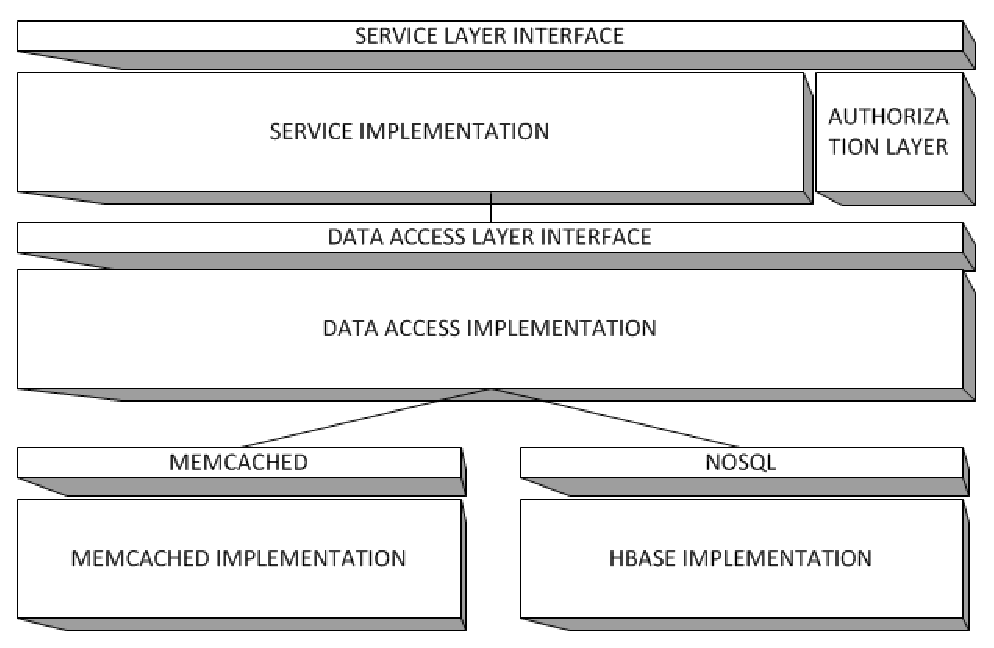
\includegraphics[width=\textwidth]{inner-arch}
  \caption{Three layers of inner architecture.}
  \label{fig:inner-arch}
\end{figure}

Service layer serves as the interface for direct or remote callings from the
application. It processes data and authorizes operations.

Data access layer fetches or stores data from/in database and transforms it
into business objects and back.

The last layer consists of basic operations like add, delete, get, replace on
database or cache and creates a simple framework over any storage.

There are four basic services currently in the application.
\begin{itemize}
\item \emph{Follow service} is responsible for creating and managing
relations. It also enables to get data about followers and following (complete
or random list which can be paginated).
\item \emph{Wall service} performs actions related to posts and walls. It
provides methods for creating, deleting and viewing either the entire post or
only minimized one (for example on wall we do not want to show all comments
connected with the post).
\item \emph{Like service} allows users to like and unlike the posts.
\item \emph{Discussion service} manages the comments of specific posts.
\end{itemize}

\subsection{Data Model}
The system consists of three tables entities, walls and discussions (their
names can be changed before initialization to avoid the problem of identical
names).

Table entities consist of five column families and saves basic information
about users. Column families followers, following and blocked contains user
ids in columns. The news column family includes post ids to the posts on news
feed (stored as a backup when Memcached fails to store news).  The last column
family count stores redundant information about numbers of followers,
following etc. so system does not have to recalculate them every time.

Table walls stores all posts of each entity in the system.  Column family info
stores basic information like author, type, number of comments and number of
likes.

In text is only one column containing the text of the post and likes contains
user ids of people who like the post.

Table discussions is very similar to the table walls but does not contain
type, likes, number of likes and comments.

\subsection{Storing Data}
While using HBase, developer has to think about row identifiers as they affect
performance. Rows are sorted lexically (identifiers are arrays of bytes) and
the only possibility how to obtain more lines is a sequence scanner, therefore
there results the need to store similar data in a batch to easily fetch them.

In table entities is user identifier (UID) the key which provides correct
sorting in other tables that uses this id as part of their keys. The key
should have constant length to ensure that data are always lexically similar.

Table walls uses concatenation of UID and time of the post (Java
SimpleDateFormat \texttt{yyyyMMddhhmmssSSS}). Thanks to that there exists only
one length of the key so posts are grouped by users and then sorted by time --
so each user has posts sorted from oldest to newest so fetching data is fast
for each user and there is higher probability that it will be stored on the
same region server.  Also users can view complete history of posts on the
wall.

In fact the posts are stored in reverse order (newest to oldest) so developer
can very fast obtain only certain number of newest posts (in the opposite
sorting it would be really hard as the scanner can read only in direction
first to last row). The solution is quite clear -- all bytes in formatted date
are inverted.

There are only weak relations among data. The entities have their posts and
they have their comments. These relations are displayed in names of keys.
Other relations are not clearly seen in the database because they are not
important.  For example user who commented our post is in database reflected
as UID but the relation with entities table is not displayed because we do not
need any data from this table (we are not interested when displaying comment
who this person follows is followed by).

\subsection{Wall and News Feed}
As is said in previous paragraph, posts are stored in table walls for each
user it is simple and fast to obtain wall for any user. The news feed is
stored in HBase only like a backup of Memcached data (for each user post
identifiers are stored so we can get the news).  Fetching the news from HBase
is relatively slow because we need to load the posts one by one.  It is the
only solution of this problem -- otherwise we would create a huge redundancy
(as many copies as many users are following). In this case Memcached can avoid
redundancy and also make access to data fast.

While sending a new post to the server all entities following user are
discovered. The post is inserted in the cache in minimized form (also time to
live is set) and link to it is put in news feed to every interested user. We
can obtain news feed in two simple cache queries. First one fetches the list
of posts and the second one (batch query) returns the posts. As Memcached is a
simple hash table in RAM getting a few posts to display is a really fast
operation.

Once the data gets old or Memcached is full the expired posts are deleted
first and after them the least recently used.

\subsection{Implementation}
System was implemented using Java EE and Spring Framework (especially
Inversion of Control and Dependency Injection principles), client libraries
for Memcached is Spymemcached developed by one of founders of Memcached and
client library for HBase is HBase 0.90.2 API for Java.

\section{Case Study}
The application was created to ensure social interactions for users of web
application Takeplace.

Takeplace \footnote{Takeplace Event Management Tool, \url{www.takeplace.eu}}
is a web-based service designed and implemented on the basis of expert
requirements for the particular tool to facilitate efficient organization of
events based on meeting, sharing and communication. Takeplace covers a wide
range of sophisticated organizational processes with unified user interface.

Users are provided with a web interface and gain an access to the standard
services for organizing events according to the type. Basic types of events
include conferences, congresses, symposia, seminars, trainings, consultation
meetings, workshops and team buildings.

In addition to the advanced organizational system, it offers its users
services like a tool for creating web presentations based on interactive
professional templates developed by experienced graphic designers, historical
continuity of given events, uniform terminology in the context of professional
event series, easy creation of promotional materials and elements of the
visual information system, assembling and typesetting proceedings and much
more.  The great advantage is the overall reduction in costs for the
management and organization of professional events and saving thus resources
otherwise needed for graphic design or spent on software equipment for
instance.

\begin{figure}[t]
  \centering
  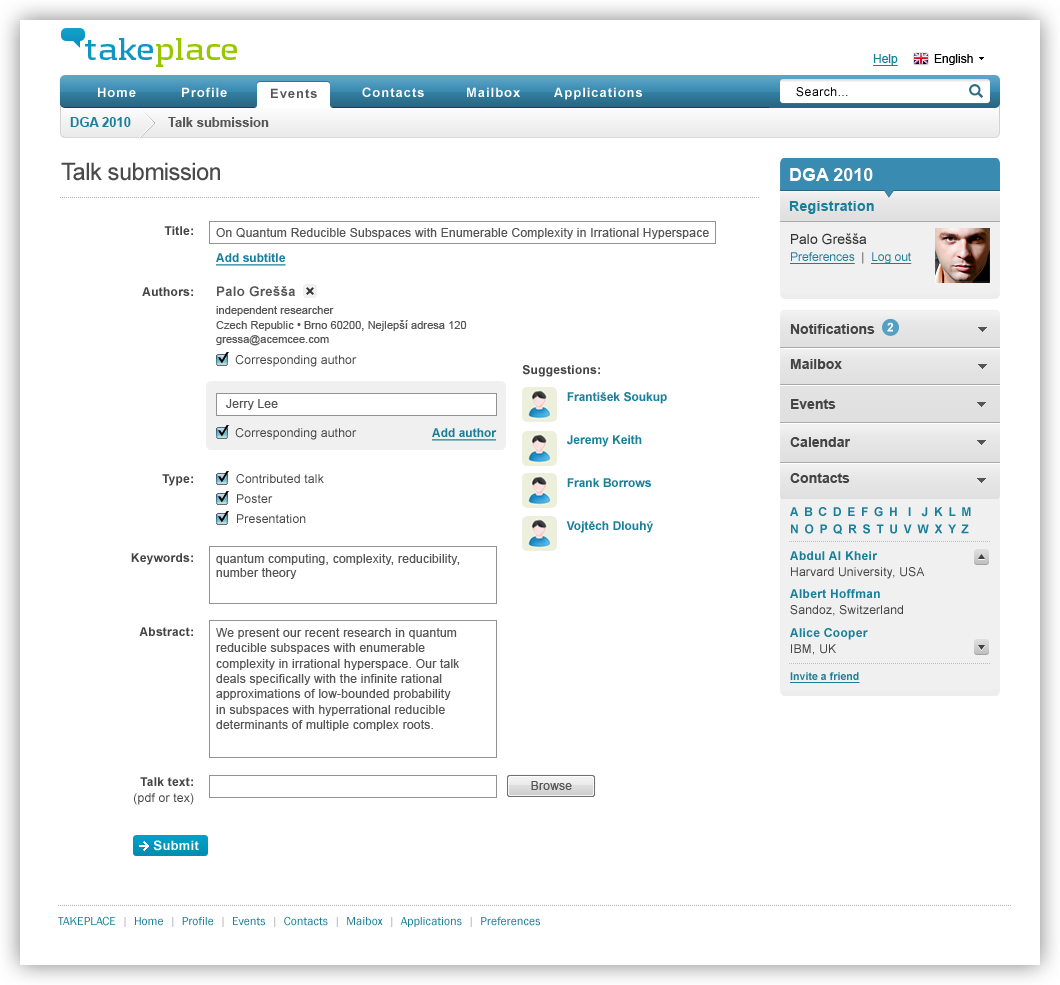
\includegraphics[width=\textwidth]{takeplace}
  \caption{Takeplace event management tool – submission.}
  \label{fig:takeplace}
\end{figure}

The Takeplace system is characterized by advanced awareness (alert subsystem)
of various aspects of the event like approaching deadlines, not receiving
outputs from involved people, exceeding quotas, etc. Thus the entire
administrative organization is considerably easy. The uniform terminology is
reached due to the historical continuity and coherence in case of annual
series of events. All events held within the system are archived and available
for visitors forever (unless they are removed by the event owner). With the
rich set of diverse functions offered, the system still has simple and
intuitive user interface (UI), exactly in the manner that Web 2.0 dictates.

Academic institutions are mainly oriented to professional training events of
greater magnitude and importance. They appreciate applications that are easy
to use and have intuitive interface, but lay emphasis on the advanced features
with formal presentation.

Finally, if the system is attractive, it increases the number of links
pointing to the web and catalyzes creation of appropriate professional users'
communities. With increasing number of professional events organized with the
Takeplace system, we will be able to evaluate these events.  Users themselves
will be able to share the experience of participation, evaluate and recommend
events to others. Then, virtual communities of professional users will arise
in course of time. The emphasis on social and interpersonal interaction is the
essential feature of Takeplace \cite{takeplace-case}.

Social network service was implemented for several reasons. One of the most
important was to provide an easy tool to comment conferences or individual
events and give a feedback to organizers and speakers.  Attenders can find
problems that hosts do not see and help them make a successful conference.
Users can also "like" events, which should compare particular seminars and
give an opportunity to people to tell which events are the best.

The second very
important reason is to create a professional user network.  Attenders of
conferences are people with common professional interests and therefore a
service allowing finding new contacts, create specialist relations and
recommend each other is needed to be implemented.

Several other use cases:
\begin{itemize}
\item Simply inform a group of people.
\item Find out how many visitors could attend particular event.
\item Hear the topics the attenders want to study.
\item Share any information among users of service.
\end{itemize}

\subsection{Implementation}
Service layer of social network service is connected with Takeplace by
communication layer that uses JSON to send needed data. Takeplace can retrieve
certain information and connects them with their database of users. User
identifiers both in the application and in the subsystem remain the same so
there is no need to transform them. Takeplace sends to the social subsystem
authenticated user id so it can authorize all needed operations.

Any data fetched from social network can be post-processed and the application
can for example after obtaining list of all followers load names and
photographs to display information. The social network subsystem independence,
easy integration and configuration are one of key features.

Succeeding step is to create graphical user interface and add more
functionality to the system (for example tagging and automatic recognition of
multimedia content).  The application was tested using unit tests, profiling
and performance tests. The subsystem has not been launched, yet, but it has
been tested on some local machines while a very simple user interface was
implemented but the real results will show in autumn 2011 when the system will
be set on production mode and opened for clients but current results look very
promising.

\section{Conclusion} The social network service was designed as a subsystem
and can be integrated into existing application by implementing the
communication layer and connect it with existing database of users.

Social module allows creating asymmetric relations among users and events.
Entities can insert posts, which can be "liked" and commented. Posts are
displayed on entity's profile wall and user can view all posts in the history.
News feed displays the newest posts from entities user is following.  The news
is stored for limited time that can be set up in configuration files.

Subsystem uses non-relational database HBase as permanent storage and
Memcached as distributed cache to improve performance, as is expected heavy
load on fetching data from database.  Non-relational database and memory cache
should decrease reading time and provide high throughput and scalability in
data-oriented web application.

Subsystem was integrated in Takeplace application and tested on local
machines.  Currently the resulting functionality is testing in a pilot run
with limited users. The availability on production servers is planed in the
end of 2011. 

\bibliographystyle{plain}
\bibliography{sofsem}

\end{document}
